%
%
%
\subsection{Characterization of electromagnetic shower properties with
a samplign calorimeter}
\label{sec:emshowerproperties}


%%
%%
%%
\subsubsection{Energy calibration and resolution}
\label{subsubsec:energyresol}

Different methods are used to measure the total energy:
\begin{itemize}
\item raw energy: simply the sum of the energy deposited in \GEANT 4 in
  the silicon in the full detector volume (30 layers of $20 \times
  20$\,cm$^2$).
\item weighted energy: sum of the energy deposited in the Si, but
  weighted differently according to which sampling section they belong
  to. Simplest weights are the ratio of sampling thicknesses in X$_0$,
  i.e. 1 for layers 0-9, 0.8/0.5 for layers 10-19 and 1.2/0.5 for
  layers 20-29. Weights can also be optimised to minimise the energy
  resolution for all energies.
\item Fit of the shower profile: allowing for example to recover the
  shower leakage for higher energies.
\end{itemize}

For the first two methods, the total energy is fitted, per incoming
energy generated, by a gaussian. The mean is used for calibration, and
the resolution is defined as the ratio of the width over the mean.

The calibration curve is shown in Figure~\ref{fig:eCalib} left, for
single electrons. Figure~\ref{fig:eCalib} right, shows the energy
resolution as a function of the incoming energy. For incoming energies
below 150 GeV, 2500 events have been generated, and 1250 above.

%@TODO replace with Pedro's plots with all 3 methods in.
\begin{figure}[h!]
  \begin{center}
%    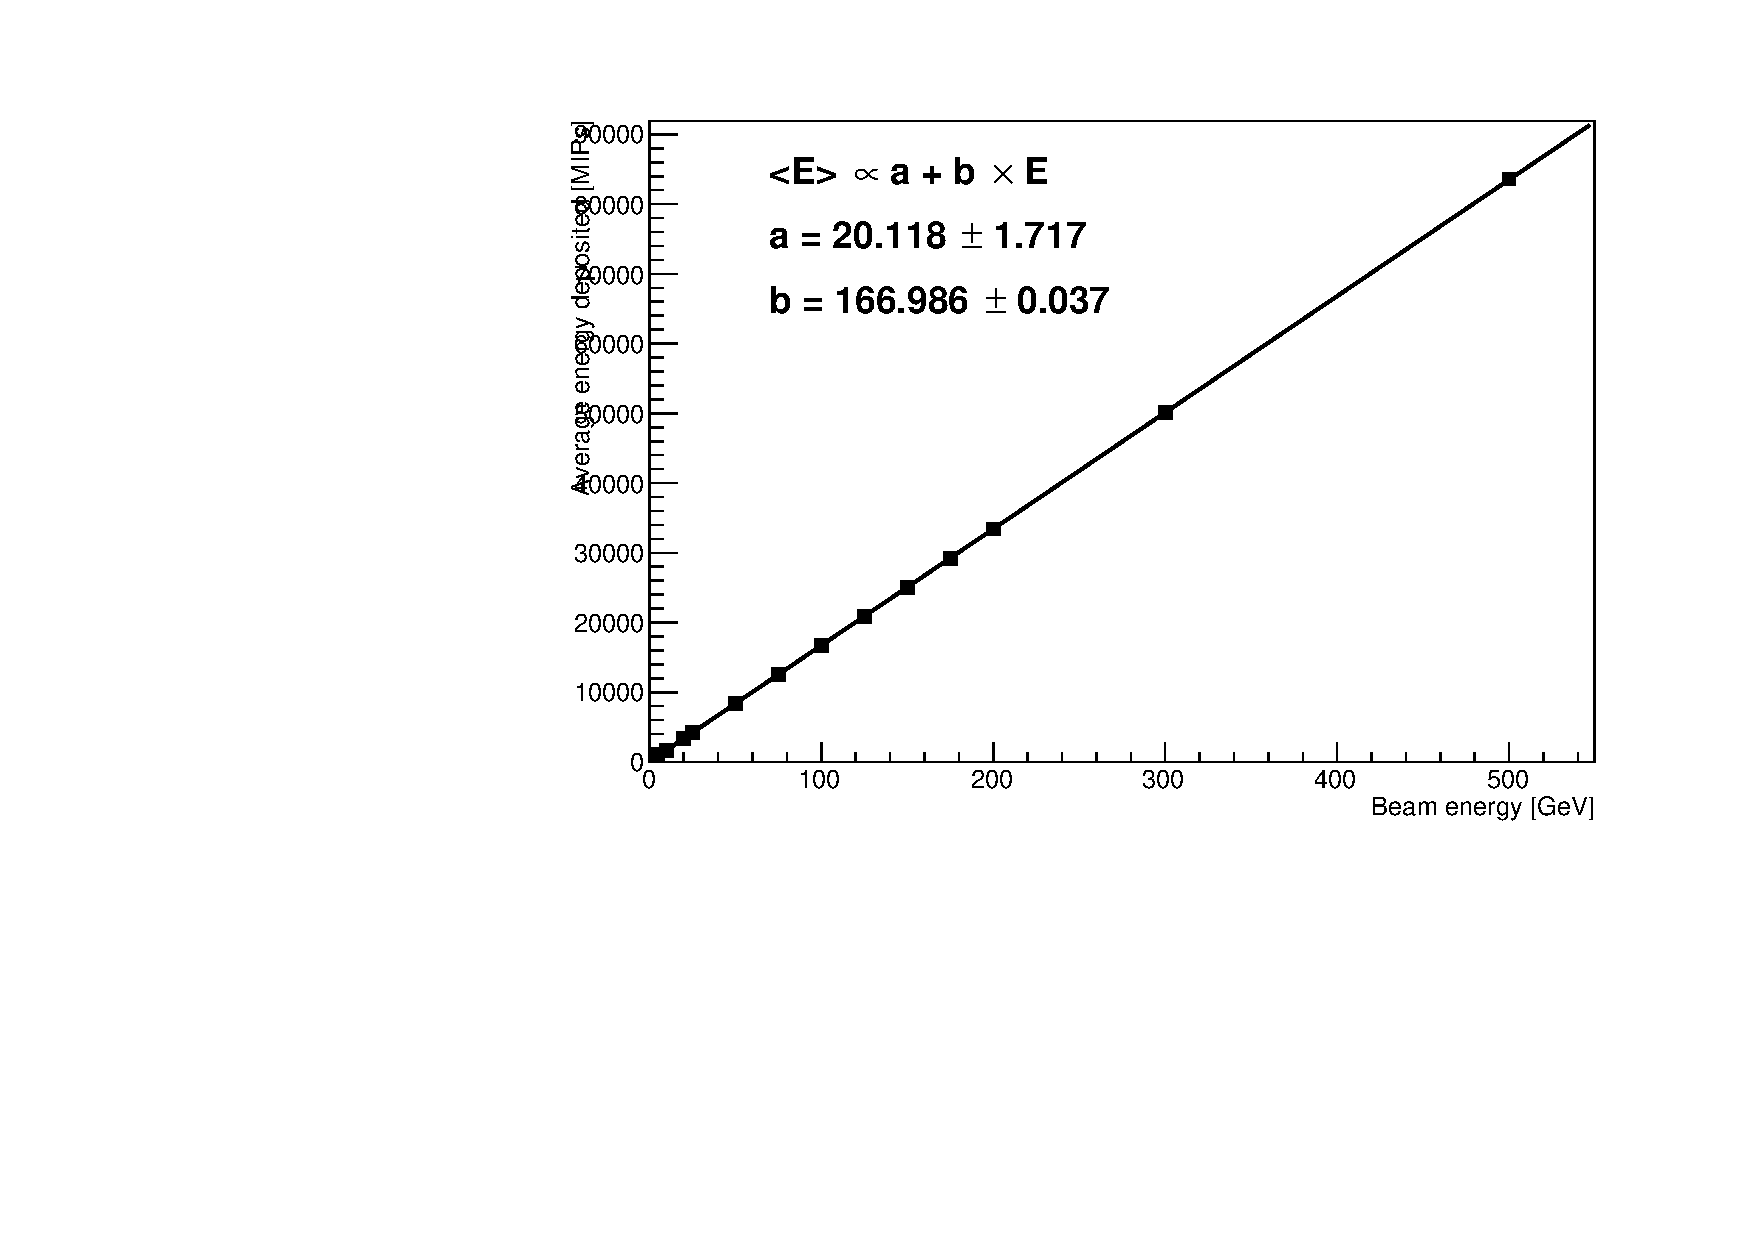
\includegraphics[width=\cmsFigWidth]{figures/e_calibFit.pdf}
 %   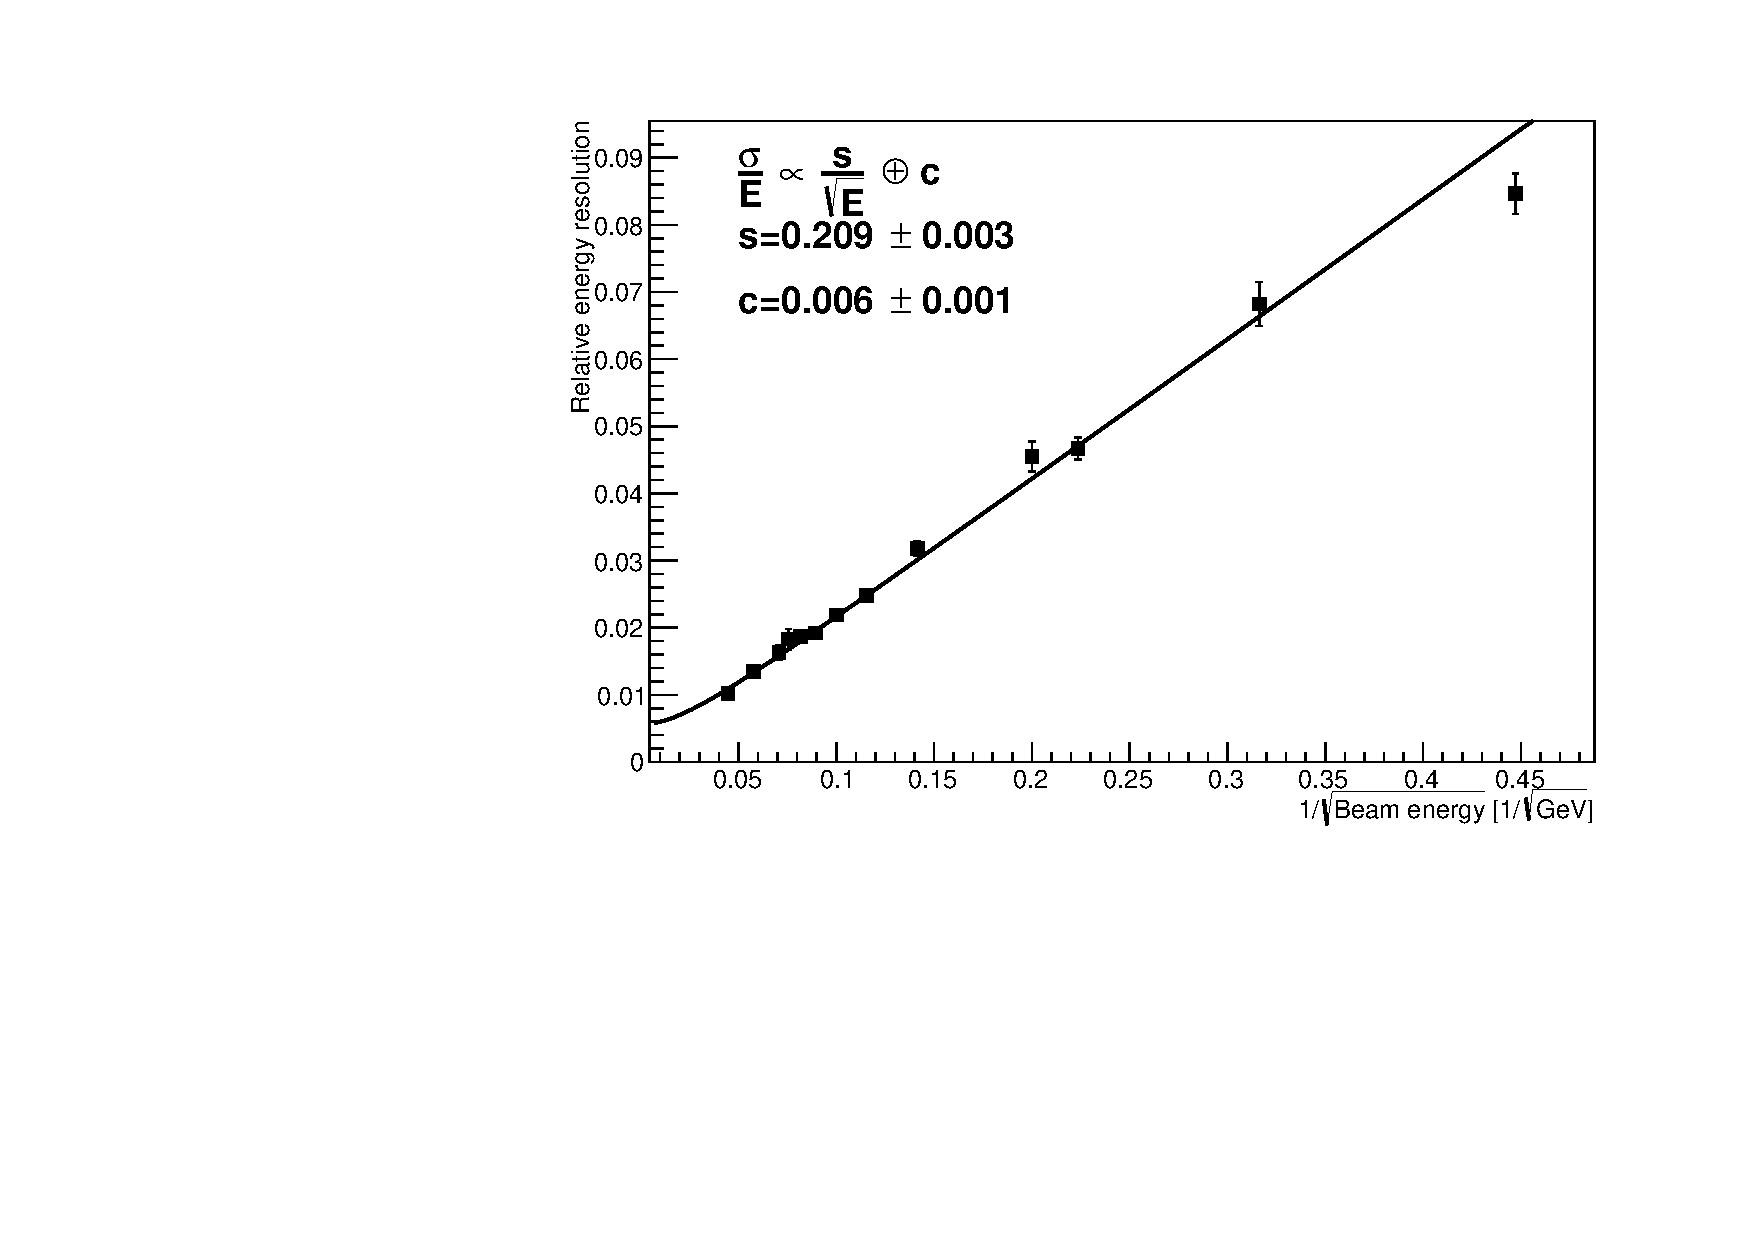
\includegraphics[width=\cmsFigWidth]{figures/e_resoFit.pdf}
    \caption{Reconstructed energy as a function of the generated
      energy E (left) and energy resolution as a function of
      $\frac{1}{\sqrt{E}}$ (right), for single electron events.}
    \label{fig:g4vis}
  \end{center}
\end{figure}
